% !TeX root = ../main.tex
\section{Цель работы и структурная схема обнаружителя}

Целью настоящей работы является исследование характеристик и имитационное моделирование устройства обнаружения радиолокационных сигналов со стабилизацией уровня ложных тревог с оценкой меньшего среднего значения (ОБН с СУЛТ-МСЗ) в гомогенных и гетерогенных помеховых условиях для заданных параметров варианта ($q = 20\text{ дБ}$, $\text{ОПШ} = 15;\; 35\text{ дБ}$, $P_{\text{лт}} = 10^{-5}$, $N = 16$, $N_G = 1$, $N_M = 3$).

Обобщенная структурная схема исследуемого обнаружителя сигналов с СУЛТ-МСЗ приведена на рисунке~\ref{fig:scheme_so_cfar}.

\begin{figure}[H]
    \centering
    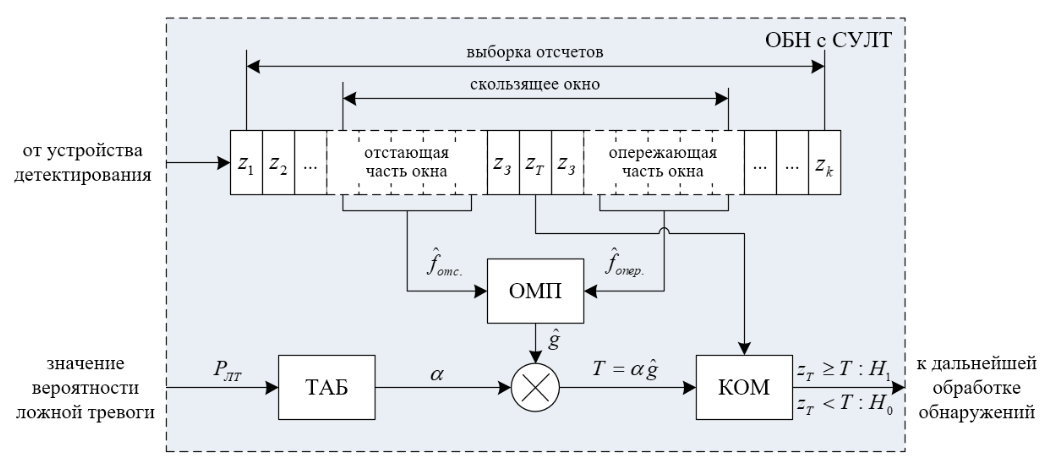
\includegraphics[width=0.85\textwidth]{export_figs/sch.png}
    \caption{Структурная схема обнаружителя сигналов с СУЛТ-МСЗ}
    \label{fig:scheme_so_cfar}
\end{figure}

В состав обнаружителя (рисунок~\ref{fig:scheme_so_cfar}) входит регистр выборки отсчетов $z_1, z_2, \dots, z_k$, поступающих с выхода квадратичного детектора. Вокруг тестируемого отсчета $z_T$ выделяются защитные ячейки $z_{\text{з}}$ ($N_G = 1$ с каждой стороны), исключающие просачивание энергии полезного сигнала в обучающую выборку, а также отстающая и опережающая части скользящего окна длиной по $N/2 = 8$ ячеек каждая. В блоке оценки мощности помехи (ОМП) вычисляются выборочные средние $\hat{f}_{\text{отс.}}$ и $\hat{f}_{\text{опер.}}$, после чего в соответствии с алгоритмом меньшего среднего значения (МСЗ) формируется результирующая оценка $\hat{g} = \min(\hat{f}_{\text{отс.}},\, \hat{f}_{\text{опер.}})$. Пороговый уровень $T = \alpha \hat{g}$ определяется путем умножения оценки $\hat{g}$ на пороговый множитель $\alpha$, выбираемый из таблицы (ТАБ) по заданному значению вероятности ложной тревоги $P_{\text{лт}}$, и подается на компаратор (КОМ) для принятия решения в пользу гипотезы наличия ($H_1$) или отсутствия ($H_0$) сигнала.

